% Section 3.5 -- Precision Refinement (role B, bonus)
\subsection{Precision Refinement}
\label{sec:B-refine}

Refinement takes the first layer from about $2^{-25}$ to about $2^{-46}$
(median), for $1200$ queries. It is needed because the row error of
Sect.~\ref{sec:B-rows} depends on the witness: a small radius or a small
$|\Atwo_j|$ gives a poor row, and that error goes straight into layer 2. The
idea is from~\cite[\S5.1]{DBLP:conf/crypto/CarliniJM20}: use the coarse row
only to find the hyperplane approximately, then locate it again with value
queries and no differencing.

For neuron $j$ we draw $x\sim\mathcal N(0,I)$, project it onto the
\emph{estimated} hyperplane, and pick a unit direction $u$ with
$|\hat a_j\cdot u|\ge0.3$. The true hyperplane is very close, so
$g(t)=f(x+tu)$ on $t\in[-\tau,\tau]$ has one kink, with
$\tau=\min(10^{-2},\tfrac12\min_{k\neq j}|\hat z_k(x)|/|\hat a_k\cdot u|)$. We do not
bisect. Two probes at each end give the left and right lines of $g$, and
their intersection $t^*$ is the kink, exact up to rounding. Two more queries
check that the midpoints of both halves lie on their lines; if not, the
point is dropped. That is $6$ queries per point and $2\dzero=20$ points per
neuron.

The snapped points lie on the true hyperplane. The normal is the right
singular vector of the centred points for the smallest singular value, and
the bias is $-\hat a\cdot\bar x'$. We drop points with residual above ten times
the median and refit once. If the row moved by more than $10^{-4}$ we keep the
old one.

Two things differ from~\cite[\S5.1]{DBLP:conf/crypto/CarliniJM20}. We bound the
segment by the estimated distance to the other hyperplanes instead of tuning
it until about half the attempts fail, and we use one round of outlier removal
instead of their robust estimator. The midpoint checks already throw out most
bad points, which is why the simpler fit is enough.

Fig.~\ref{fig:B-refine} tests refinement alone: Gaussian noise with standard
deviation $10^{-8}$ on the true, normalised first layer of 100 $U[0,1]$
networks. The maximum parameter error goes from a median of $2^{-25.2}$ to
$2^{-46.1}$; the worst network ends at $2^{-39.0}$, and $99\%$ reach $2^{-40}$.
With noise $10^{-6}$ or $10^{-10}$, and for $U[-1,1]$ and $\mathcal N(0,1)$
weights, $96$--$100\%$ reach $2^{-40}$ and the worst case is $2^{-36.3}$
(\texttt{results/b\_refine.csv}). How coarse the input was does not matter,
as long as the true hyperplane falls inside the short segment.

\begin{figure}[t]
\centering
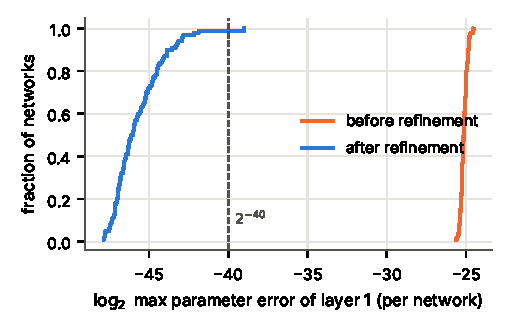
\includegraphics[width=0.75\linewidth]{figures/B/b_refine.pdf}
\caption{Distribution over 100 $U[0,1]$ networks of the largest first-layer
parameter error before and after refinement (input noise $10^{-8}$).}
\label{fig:B-refine}
\end{figure}
